\documentclass[12pt]{article}
\usepackage[utf8]{inputenc}
\usepackage{amsxtra}
\usepackage{amssymb}
\usepackage{amsthm}
\usepackage{latexsym}
\usepackage{graphicx}
\usepackage{imakeidx}
\usepackage{booktabs}
\usepackage{tikz}

\title{\textbf{Sheet 01 - Solution}}
\author{Terrible Island}
\date{November 26th 2019}

\begin{document}

\maketitle

\setlength{\baselineskip}{0.6cm}

\section{Question 1}

\textbf{a)} Let $G = (V,E)$ be a graph, let $S \subset E$, and let $M_{G}$ be the spanning tree matroid associated to $G$. We'll show $M_{G}/S = M_{G/S}$ by proving it for the case of a single edge, $e \in E$, and the general case of a set of edges $S$ will follow by induction.

Let $e \in E$ be a loop. Then, $e \notin I : \forall I \in M_{G}$, thus $G/e = G \setminus e$. Therefore, since all $I \in M_{G}$ behave in the same manner: $$M_{G}/e = M_{G} \setminus e = M_{G \setminus e} = M_{G/e}$$

Suppose $e$ is not a loop, and let $I \subset E \setminus \lbrace e \rbrace$. We'll firstly show that $I \cup \lbrace e \rbrace$ has a cycle if, and only if, $I$ contains a cycle of $G/e$. Indeed: let $I \cup \lbrace e \rbrace$ contain a cycle (in $G$). Then, if $e$ is in the cycle, both ends of it are identified in $G/e$, and the cycle remains as such in $G/e$; if $e$ is not in the cycle, then the cycle remains identical in $G/e$, therefore if $I \cup \lbrace e \rbrace$ contains a cycle, $I$ contains a cycle in $G/e$. On the other hand, suppose $I \cup \lbrace e \rbrace$ does not have a cycle in $G$. Then, at least one of the ends of $e$ is a vertex that is not an end of any other edge in $I$ (informally, a vertex outside of $I$). Therefore, $I$ cannot have a cycle when contracting by $e$, since if a cycle were to be created by the contraction, both ends of $e$ would be ends of edges in $I$.

With this, we conclude $M_{G}/e = M_{G/e}$, and as said in the beginning, this inductively implies $M_{G}/S = M_{G/S}$.

\textbf{b)} Let $I$ be an independent set of the matroid M, which for the sake of simplicity we'll write as $I \in M$, and let $e \in [n]$. We have that: $$I \in M \Leftrightarrow \ [n] \setminus I \in M^{*} \Rightarrow ([n] \setminus \lbrace e \rbrace) \setminus (I \setminus \lbrace e \rbrace ) \in M^{*} \setminus \lbrace e \rbrace \Rightarrow$$ $$\Rightarrow I \setminus \lbrace e \rbrace \in (M^{*} \setminus \lbrace e \rbrace ) ^{*}$$ 
Thus the two notions of contraction agree in the case of one element, which by induction means they agree on the contraction of any finite collection of said elements.

\textbf{c)} We will provide an explicit correspondence between the basis of $M_{G^{*}}$ and $M_{G}^{*}$. Let $n, m, f \in \mathbb{N}$ be the numbers of vertices, edges, and faces of the planar graph $G$, and let $n', m', f' \in \mathbb{N}$ be those of its dual (by definition, also a planar graph). Let $T$ be a spanning tree of $G$, which has $n-1$ edges, and let $T^{*}$ be its dual, which will have $t^{*} = m-n+1$ edges. By Euler's formula ($n-m+f=2$): 

$$n' = f = 2-n+m \ , \ t^{*} = m-n+1 \Rightarrow$$ $$\Rightarrow t^{*}= n'-1$$

So $T^{*}$ has $n'-1$ edges, thus if it's acyclic, it will be a spanning tree. Suppose $T^{*}$ has a cycle. This cycle encloses a face of $G^{*}$, which corresponds to a vertex of $G$. The edges of $T^{*}$ correspond to edges in the complementary of $T$ in $G$, thus the vertex corresponding to the face enclosed by the cycle in $G$ has no edge of $T$ connecting it to the rest of the spanning tree, against what a spanning tree is. We have contradiction, thus $T^{*}$ cannot have a cycle, and is therefore a spanning tree of $G^{*}$.

This mapping is injective, since if two trees have the same dual they coincide edge by edge, thus they are equal. It's also surjective, since applying the mapping from $G^{*}$ to $G$ provides an inverse. Therefore, we have equality between the matroids.

\textbf{d)} Let us have the matrix:$$A = \left( {\begin{array}{ccccc}
   0 & 1 & 1 & 0 & 1\\
   1 & 0 & 1 & 0 & 1\\
   0 & 1 & 1 & 1 & 0\\
  \end{array} } \right)$$

Swapping columns 1 and 2, and 3 and 4, we obtain: $$\left( {\begin{array}{ccccc}
   1 & 0 & 0 & 1 & 1\\
   0 & 1 & 0 & 1 & 1\\
   1 & 0 & 1 & 1 & 0\\
  \end{array} } \right)$$
  
And substracting row 1 to row 3 we obtain: $$A_{1} = \left( {\begin{array}{ccccc}
   1 & 0 & 0 & 1 & 1\\
   0 & 1 & 0 & 1 & 1\\
   0 & 0 & 1 & 0 & -1\\
  \end{array} } \right)$$
  
 Which is in the form $A_{1} = (Id_{3} | B)$. Now, let $A_{1}^{*} = (-B^{t} | Id_{2})$:  $$A_{1}^{*} = \left( {\begin{array}{ccccc}
   -1 & -1 & 0 & 1 & 0\\
   -1 & -1 & 1 & 0 & 1\\
  \end{array} } \right)$$
  
Then, $A_{1}A_{1}^{*t} = 0$, and by the previous exercise, it's the matrix realization of the dual matroid with certain elements swapped. We can observe that the realisation given by $A_{1}$ (and by $A$, since they'll be isomorphic) corresponds to the graphical matroid of the graph \ref{figura1}, and its dual to the graph \ref{figura2}, which indeed satisfies that $A_{1}^{*}$ is a representation of.

\begin{figure}
    \centering
    \includegraphics{figures/figura1.JPG}
    \caption{Graph with graphical matroid represented by $A_{1}$, isomorphic to that represented by $A$}
    \label{figura1}
\end{figure}

\begin{figure}
    \centering
    \includegraphics{figures/figura2.JPG}
    \caption{Graph with graphical matroid represented by $A_{1}^{*}$, dual to the one in \ref{figura1}}
    \label{figura2}
\end{figure}

Let us consider the contraction on column 1 of $A$, which corresponds to column $2$ in $A_{1}$, and edge $b$ in graph \ref{figura1}. This corresponds to the dual of the deletion of column 2 from the dual matroid $A_{1}^{*}$. In particular: $$A_{1}^{*} \setminus b = \left( {\begin{array}{cccc}
   -1 & 0 & 1 & 0\\
   -1 & 1 & 0 & 1\\
  \end{array} } \right)$$
  
$$A_{1} \setminus b = (A_{1}^{*} \setminus b)^{*} = \left( {\begin{array}{ccccc}
   1 & 1 & 1 & 0\\
   0 & -1 & 0 & 1\\
  \end{array} } \right)$$
  
Which, indeed, is a realisation of the graphical matroid of graph \ref{figura1} contracted on $b$ (graph \ref{figura3}).

\begin{figure}
    \centering
    \includegraphics{figures/figura3.JPG}
    \caption{Contraction of graph \ref{figura1} on the edge $b$}
    \label{figura3}
\end{figure}

\section{Question 2}

Let $A \in Mat_{d \times n}$ and $B \in Mat_{n \times n-d}$ be matrices such that $AB = 0$. We'll show that: $$LinVal(B^{t}) = LinDep(A)$$

We define those two sets as: $$LinVal(A) = \lbrace v^{t}A : v \in \mathbb{R}^{d} \rbrace = im(A^{t}) \subseteq \mathbb{R}^{n}$$ $$LinDep(A) = \lbrace v \in \mathbb{R}^{n} | Av = 0 \rbrace = ker(A)$$

Let $v \in LinVal(B^{t}) \subseteq \mathbb{R}^{n}$. Then, there exists $w \in \mathbb{R}^{n-d}$ such that $v^{t} = w^{t}B^{t}$, which is equivalent to $v = Bw$. Therefore, $Av = ABw = 0w = 0$, hence $v \in LinDep(A)$ and $LinVal(B^{t}) \subseteq LinDep(A)$.

To see that we have equality, we observe that $A$ has full rank, $d$, thus considering it as a linear map $A : \mathbb{R}^{n} \longrightarrow \mathbb{R}^{d}$, its image has dimension $d$ and its kernel dimension $n-d$. On the other hand, $B$ also has full rank $n-d$ since it's a Gale transform of A, thus $im(B) = LinVal(B^{t})$ also has dimension $n-d$. As both are linear subspaces of $\mathbb{R}^{n}$ of the same dimension, and one is contained in the other, they must be equal.

\section{Question 3}

\textbf{a)} We'll show it by induction. Our induction hypothesis will be that $w(K)\geq w(P)$ if they have $n$ or less elements not in common where $K$ is the Kruskal solution and $P$ an optimal solution.

For our \textbf{ground case}, let $k$ the first, and unique element of $K$ that is not in $P$ and $p$ the element that is not in $K$. When $k$ was considered in the algorithm $p$ was also considered and that implies $w(k)\geq w(p)$ and given the fact that $K$ and $P$ only differ in one element we conclude $w(K)\geq w(P)$.

Suppose our induction hypothesis holds for the case $n$. In the \textbf{case $n+1$}, let $p$ the last element of $P$ that is not in $K$, using the exchange axiom we know that exists $k \in K-P$ such that $P'=P- \lbrace p \rbrace \ \cup \lbrace k \rbrace$ is a basis. Now notice the following: given the fact that $P'$ is a basis when $k$ was considered in the algorithm $p$ was also considered and that implies that $w(P)\leq w(P')$ and, by our induction hypothesis, $w(P')\leq w(K)$. With this, we conclude the induction holds.

\textbf{b)} We'll see that the exchange axiom holds. Let $I_{1}, I_{2} \in \mathcal{I}$ with $|I_{1}|=|I_{2}|+1=k+1$. Consider the weight function:
$$
w(e)=
\begin{cases}
\frac{k+1}{k+2} & e\in I_{1}\\
\frac{k}{k+1} & e\in I_{2} \setminus I_{1}\\
0 & \text{otherwise} 
\end{cases}
$$

Notice that the greedy algorithm will take all the elements of $I_{1}$ in the solution because they are independent and have the biggest associated weight. Once all the elements of $I_{1}$ are chosen, the total weight of the set is $\frac{k+1}{k+2}k$, now given the fact that the algorithm always works and $I_{2}$ is a feasible solution with  total weight $\frac{k}{k+1}(k+1)=k>\frac{(k+1)k}{k+2}$ at least one element of $I_{2}$ will be chosen by the algorithm. We conclude that exists an element $i\in I_{2} \setminus I_{1}$ such that $I_{1} \cup \lbrace i \rbrace$ is an independent set.

\section{Question 4}

\textbf{a)} Let $I_{1}, I_{2}$ be independent sets in $M_{1}, M_{2}$. Firstly, we can observe that their intersection is a matching, since $e \in I_{1} \cap I_{2}$ has no vertex in common with any other edge in the intersection (since $I_{1}$ discards common vertices in $V_{1}$, and $I_{2}$ in $V_{2}$). Note as well that any matching is an independent set in both $M_{1}$ and $M_{2}$, thus the maximum size of a matching is the maximum size of an intersection of independent sets. Therefore, by the \textit{Matroid Intersection Theorem}, the maximum size of a matching is equal to $min \lbrace r_{1}(S) + r_{2}(E \setminus S) : S \subseteq E \rbrace$.

Let $S \subseteq E$, and let $I_{1} \in M_{1}$ and $I_{2} \in M_{2}$ be such that: $$|I_{1}| = r_{1}(S) \ , \ I_{1} \subseteq S$$ $$|I_{2}| = r_{2}(E \setminus S) \ , \ I_{2} \subseteq (E \setminus S)$$

Let $S_{1} \subseteq V_{1}$ be the set of vertices of $V_{1}$ with at least an edge in $S$, and let $S_{2} \subseteq V_{2}$ be the set of vertices of $V_{2}$ with at least an edge in $E \setminus S$. Clearly, $e \in I_{1} \cap I_{2}$ has one vertex in $S_{1}$ and one vertex in $S_{2}$, and in fact, $|S_{i}| = |I_{i}|$, thus $r_{1}(S) + r_{2}(E \setminus S) = |S_{1} \cup S_{2}|$

We can show $S_{1} \cup S_{2}$ is a vertex cover. Let $e \in E$ be an edge. If $e \in S$, then there is a vertex $v_{1} \in S_{1}$ such that $e = \lbrace v_{1}, v \rbrace$. If $e \notin S$, then there exists $v_{2} \in S_{2}$ such that $e = \lbrace v_{2}, v \rbrace$. Therefore, all vertices in $E$ are covered by $S_{1} \cup S_{2}$, thus it's a vertex cover, whose minimum size corresponds to the minimum sum of the ranks in the \textit{Matroid Intersection Theorem}, which coincides with the maximum size of a matching in the graph.

\textbf{b)} Let $M_{1}$ be the cycle matroid of $G$, $M_{2}$ be the transversal matroid of $G$ on the partition given by the $k$ colours, and let $n$ be the number of vertices of $G$. Then, if we define a \textit{rainbow forest} as a forest in $G$ where no two edges are the same colour, it's clear that for every $I_{1} \in M_{1}$ and $I_{2} \in M_{2}$, $I_{1} \cap I_{2}$ is a rainbow forest. Therefore, there exists a rainbow tree in $G$ if, and only if: $$max \lbrace |I_{1} \cap I_{2} | \ : \ I_{i} \in M_{i} \rbrace = n-1$$

On the other hand, we can observe that, for every $S \subseteq E$, $r_{1}(S)$ is the largest forest of $G$ in $S$, and $r_{2}(S)$ is the number of different colours in $S$. 

Let $F \subseteq E$ be a union of $t \geq 0$ colours, which without loss of generality we can suppose to be $F = E_{1} \cup ... \cup E_{t}$. Suppose $G \setminus F$ has, at most, $t+1$ connected components. We can firstly observe that $G$ is then connected, since then: $$t=0 \Rightarrow F = \emptyset \Rightarrow G \text{has at most one connected component}$$

Let $S = E \setminus F$. Then, $r_{1}(S)$ is the number of edges in the largest forest in $G \setminus F$, which is a spanning forest (union of the spanning trees of each connected component), whose size is, at least, $n-t-1$, and $r_{2}(E \setminus S) = r_{2}(F) = t$. Therefore, $r_{1}(S) + r_{2}(E \setminus S) \geq n-1$. This is actually a lower bound to that sum of ranks, since for any $e \in F$, if we take $S = E \setminus (F \setminus \lbrace e \rbrace )$ (assuming it does not affect the number of colours either), either $e$ does not affect the number of connected components, so the sum does not change, or it lowers the number of connected components by one, obtaining $r_{1}(S) + r_{2}(E \setminus S) = n > n-1$. Therefore, the minimum is $n-1$, and by the \textit{Matroid Intersection Theorem}: $$n-1 = max \lbrace |I_{1} \cap I_{2} | \ : \ I_{i} \in M_{i} \rbrace$$

Thus there exists a rainbow spanning tree.

Suppose, now, that there exists some $t \geq 0$ such that $G \setminus F$ has at least $t+2$ connected components. Then, defining $S = E \setminus F$ as before, $r_{2}(E \setminus S) = t$ again, but $r_{1}(S) \leq n-t-2$. Therefore, $min \lbrace r_{1}(S) + r_{2}(E \setminus S) \ : \ S \subseteq E \rbrace \leq n-2$, so by the \textit{Matroid Intersection Theorem}, there cannot be any rainbow spanning tree, since every rainbow forest has, at most, $n-2$ edges.

\section{Question 5}

We'll firstly show that graphical matroids are realisable. Let $G=(E,V)$ be a graph, and $\mathbb{K}^{|V|}$ a vector space with canonical basis $\{e_{v}\}$, indexed by the vertices of the graph. Now let's consider for each edge $\{v,w\}$ the vector $e_{v}-e_{w}$. Let's prove that a set of edges contains a cycle if, and only if, there exists a linear dependence amongst the vectors corresponding to the edges of said set of vertices.

Let $B$ be a set of edges that contains a cycle, $C$. Consider the sum of the vectors corresponding to the edges of the cycle $C$:
$$
\sum_{\{u,w\}\in C}v_{u,v}=e_{v_{1}}-e_{v_{2}}+e_{v_{2}}-e_{v_{3}}\ldots+e_{v_{n}}-e_{v_{1}}=0
$$
Which vanishes because it's a telescopic sum.

Suppose that there is no cycle in the graph, and consider a path in $G$. We'll show that the vectors of the edges of the path are independent. The path cannot start and end with the same vertex, since it's a subset of vertices of a tree. Suppose there is a vanishing linear combination:
$$
\sum_{i=1}^{n}\alpha_{i}v_{i}=\alpha_{1}(e_{1}-e_{2})+\ldots+\alpha_{n}(e_{n-1}-e_{n})=0
$$

The vector $e_{1}$ only appears once, so to be cancelled we need $\alpha_{1}=0$ and with the same argument we can argue that $\alpha_{i}=0$ $\forall i\in\{1,\ldots,n\}$. So the only way the linear combination vanishes is that all the coefficients are null, which implies that a path in $G$ is independent.

Now, we'll show transversal matroids are realisable. Consider a bipartite graph $G=(A\cup F,E)$, and the following matrix indexing the columns by the vertices of $A$ and the rows by the vertices of $F$. Let the matrix be in the field $\mathbb{K}(X)$.
$$
\begin{pmatrix}
x_{1,1} & 0 & x_{1,3} & x_{1,4} & 0 & x_{1,6}\\
 x_{1,2} & x_{2,2} & 0 & x_{2,4} & 0 & x_{2,6}\\
 0 & x_{3,2} & x_{3,3} & 0 & x_{3,5} & 0\\
\end{pmatrix}
$$
Where there is an transcendent element of $\mathbb{K}$ if there is an edge connecting the two vertices. Note that, in this example, we have $|F|=3$ and $|A|=6$. Suppose without loss of generality that $|A|>|F|$ and let $B \subseteq A$. Let's prove firstly that if $|B|>|F|$ (that implies dependent set in the matroid), then the vectors corresponding to the set of vertices $B$ are dependent. The vectors are understood as vectors of the $\mathbb{K}(X)$-vector space $\mathbb{K}(X)^{|F|}$ where $K(X)=k(x_{i,j}|{i,j}\in E)$. The dimension of this vector space is $|F|$, so if we consider more than $|F|$ vectors these vectors have to be dependent.

Now let's prove that if we consider $|B|=|F|$ then $B$ is a dependent set if, and only if, the determinant of the submatrix whose vectors are the ones corresponding with $B$ is equal to $0$.

If $B$ is a dependent set, that will mean that there is no matching between the elements of $B$ and $F$. That means that, if we consider a permutation on the elements by columns, it always contains a $0$, and the determinant is the sum of the product of every permutation. Since every permutation contains a $0$ that will mean the determinant is equal to $0$.

Let's prove that if the determinant equal $0$ implies $B$ dependent. The claim is if the determinant is equal to $0$, that will mean every permutation has at least a $0$, because if not we can construct a polynomial in $K(X\mathrm{/} x_{i,j})$ that vanishes $x_{i,j}$ and contradicts the fact that $x_{i,j}$ is transcendent. So if the determinant is $0$, that implies there is a $0$ in every permutation, which means there is no matching between $B$ and $F$, implying $B$ dependent.

In conclusion, every transversal matroid is realizable

\section{Question 10}

\textbf{a)} Consider the following matrix:
$$
\begin{pmatrix}
1 & 0 & 0 & 1 & 1 & 0 & \gamma\\
0 & 1 & 0 & 1 & 0 & \alpha & \delta\\
0 & 0 & 1 & 0 & 1 & \beta & \epsilon
\end{pmatrix}
$$
where every column corresponds to an element of the matroid in alphabethic order, and all the parameters are not $0$
It's easy to check that if you consider a triangle in any of the two matroids it corresponds to maximal independent set of the vectors column of the matrix. So we can deduce that this two matrods are realizable in a matrix of ths form.

\textbf{b)} We know that the set of elements $\{2,7,6\}$ is dependent, thus we have:
$$
\alpha_{1}(0,0,1)+\alpha_{2}(1,1,0)+\alpha_{3}(\gamma,\delta,\epsilon)=0
$$
We deduce from this equality that $\gamma=\delta$.
We also know that the elements $\{4,7,3\}$ is dependent, then we have:
$$
\alpha_{1}(0,1,0)+\alpha_{2}(1,0,1)+\alpha_{3}(\gamma,\delta,\epsilon)=0
$$
We deduce from the two equalities $\gamma=\delta=\epsilon$.

\textbf{c)} We know that the set of elements $\{1,7,5\}$ are dependent, therefore we have:
$$
\alpha_{1}(1,0,0)+\alpha_{2}(\gamma,\delta,\epsilon)+\alpha_{3}(0,\alpha,\beta)=0
$$
From this equality we know that  $\alpha_{3}\beta=\alpha_{2}\epsilon=\alpha_{2}\delta=\alpha_{3}\alpha\rightarrow\beta=\alpha$

\textbf{d)} In the first matroid we see that the set $\{4,5,6\}$ is dependent so we have:
$$
\alpha_{1}(1,1,0)+\alpha_{2}(1,0,1)+\alpha_{3}(0,\alpha,\beta)=0
$$
from here we deduduce that $\alpha_{1}=-\alpha_{2}$, from here we deduce that $\alpha_{1}+\alpha_{3}\beta=-\alpha_{1}+\alpha_{3}\beta=0\rightarrow \alpha=-\alpha$ with $\alpha\neq 0$ that tells us $1=-1$ and that implies that $\mathbb{K}$ is of characteristic $2$.

In the second matroid we can use the same argument tot say that if $\mathbb{K}$ is of charecteristic $2$ we can a linear combination of the vector corresponding to $\{4,5,6\}$ equals to the zero vector and that's not possible because in the second matroid $\{d,e,f\}$ are independent

\section{Question 12}

We have 6 points in dimension 0, which means we are in $6-0-2=4$-dimensional space. We will go from the affine Gale diagram to the Gale diagram. 


\begin{itemize}
\item Four  positive points, two negative points.
\begin{figure}
\centering
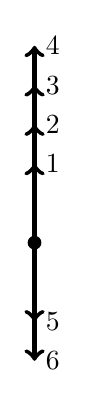
\begin{tikzpicture}
\draw[->,ultra thick](0,0) -- (0,1) node[anchor=west]{1};
\draw[->,ultra thick](0,0) -- (0,1.5)node[anchor=west]{2};
\draw[->,ultra thick](0,0) -- (0,2)node[anchor=west]{3};
\draw[->,ultra thick](0,0) -- (0,2.5)node[anchor=west]{4};
\filldraw (0,0) circle (0.08cm);
\draw[->,ultra thick](0,0) -- (0,-1)node[anchor=west]{5};
\draw[->,ultra thick](0,0) -- (0,-1.5)node[anchor=west]{6};
\end{tikzpicture}\hspace{1cm}
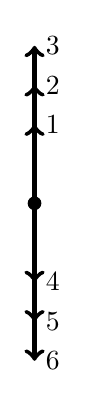
\begin{tikzpicture}
\draw[->,ultra thick](0,0) -- (0,1) node[anchor=west]{1};
\draw[->,ultra thick](0,0) -- (0,1.5)node[anchor=west]{2};
\draw[->,ultra thick](0,0) -- (0,2)node[anchor=west]{3};
\filldraw (0,0) circle (0.08cm);
\draw[->,ultra thick](0,0) -- (0,-1)node[anchor=west]{4};
\draw[->,ultra thick](0,0) -- (0,-1.5)node[anchor=west]{5};
\draw[->,ultra thick](0,0) -- (0,-2)node[anchor=west]{6};
\end{tikzpicture}\hspace{1cm}
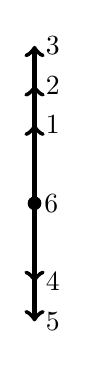
\begin{tikzpicture}
\draw[->,ultra thick](0,0) -- (0,1) node[anchor=west]{1};
\draw[->,ultra thick](0,0) -- (0,1.5)node[anchor=west]{2};
\draw[->,ultra thick](0,0) -- (0,2)node[anchor=west]{3};
\filldraw (0,0) circle (0.08cm) node[anchor=west]{6};
\draw[->,ultra thick](0,0) -- (0,-1)node[anchor=west]{4};
\draw[->,ultra thick](0,0) -- (0,-1.5)node[anchor=west]{5};
\end{tikzpicture}\hspace{1cm}
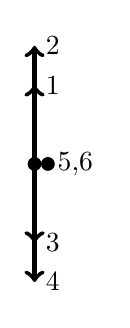
\begin{tikzpicture}
\draw[->,ultra thick](0,0) -- (0,1) node[anchor=west]{1};
\draw[->,ultra thick](0,0) -- (0,1.5)node[anchor=west]{2};
\filldraw (0,0) circle (0.08cm);
\filldraw (0.17,0) circle (0.08cm) node[anchor=west]{5,6};
\draw[->,ultra thick](0,0) -- (0,-1)node[anchor=west]{3};
\draw[->,ultra thick](0,0) -- (0,-1.5)node[anchor=west]{4};
\end{tikzpicture}
\caption{From left to right, \{4,2\},\{3,3\},\{3,2,1\},\{2,2,2\}.}
\end{figure}

\begin{figure}[h]
\centering
\begin{tabular}{cccccc}
1 & 2 & 3 & 4 & 5 & 6 \\ \hline
+ & 0 & 0 & 0 & + & 0 \\
+ & 0 & 0 & 0 & 0 & + \\
0 & + & 0 & 0 & + & 0 \\
0 & + & 0 & 0 & 0 & + \\
0 & 0 & + & 0 & + & 0 \\
0 & 0 & + & 0 & 0 & + \\
0 & 0 & 0 & + & + & 0 \\
0 & 0 & 0 & + & 0 & +
\end{tabular}
\caption{Facets of \{4,2\}.}
\end{figure}
\begin{figure}
\centering
\begin{tabular}{cccccc}
1 & 2 & 3 & 4 & 5 & 6 \\ \hline
+ & 0 & 0 & + & 0 & 0 \\
+ & 0 & 0 & 0 & + & 0 \\
+ & 0 & 0 & 0 & 0 & + \\
0 & + & 0 & + & 0 & 0 \\
0 & + & 0 & 0 & + & 0 \\
0 & + & 0 & 0 & 0 & + \\
0 & 0 & + & + & 0 & 0 \\
0 & 0 & + & 0 & + & 0 \\
0 & 0 & + & 0 & 0 & +
\end{tabular}
\caption{Facets of \{3,3\}.}
\end{figure}

\begin{figure}
\centering
\begin{tabular}{cccccc}
1 & 2 & 3 & 4 & 5 & 6 \\ \hline
+ & 0 & 0 & + & 0 & 0 \\
+ & 0 & 0 & 0 & + & 0 \\
0 & + & 0 & + & 0 & 0 \\
0 & + & 0 & 0 & + & 0 \\
0 & 0 & + & + & 0 & 0 \\
0 & 0 & + & 0 & + & 0 \\
0 & 0 & 0 & 0 & 0 & +
\end{tabular}
\caption{Facets of \{3,2,1\}.}
\end{figure}

\begin{figure}
\centering
\begin{tabular}{cccccc}
1 & 2 & 3 & 4 & 5 & 6 \\ \hline
+ & 0 & + & 0 & 0 & 0 \\
+ & 0 & 0 & + & 0 & 0 \\
0 & + & + & 0 & 0 & 0 \\
0 & + & 0 & + & 0 & 0 \\
0 & 0 & 0 & 0 & + & 0 \\
0 & 0 & 0 & 0 & 0 & +
\end{tabular}
\caption{Facets of \{2,2,2\}.}
\end{figure}

\end{itemize}
\end{document}